% ===================================================================
% Resultados de evaluación (val y test) --- versión reducida
% Números: checkpoints/*_{val,test}_metrics.json
% Figuras de resultados: figures/ (regenerar con make_figures.py)
% Figuras de contexto:   ../../research/figures/
% Compilar: cd docs/presentations && latexmk -pdf resultados_evaluacion.tex
% ===================================================================
\documentclass[aspectratio=169,10pt]{beamer}

\usepackage[utf8]{inputenc}
\usepackage[T1]{fontenc}
\usepackage[spanish,es-tabla,es-noquoting]{babel}
\usepackage{booktabs}
\usepackage{array}
\usepackage{graphicx}
\usepackage{xcolor}
\usepackage{amsmath}

\usetheme{metropolis}
\metroset{numbering=fraction, progressbar=frametitle, block=fill, sectionpage=none}

% Paleta: la misma de las figuras, para que texto y marcas coincidan.
\definecolor{cFRCNN}{HTML}{2A78D6}
\definecolor{cDETR}{HTML}{EB6834}
\definecolor{cDETRb}{HTML}{1BAF7A}
\definecolor{cYOLO}{HTML}{4A3AA7}
\definecolor{cInk}{HTML}{0B0B0B}
\definecolor{cMuted}{HTML}{52514E}
\setbeamercolor{frametitle}{bg=cInk}
\setbeamercolor{progress bar}{fg=cFRCNN}

\newcommand{\gris}[1]{{\color{cMuted}#1}}
\newcommand{\frcnn}{{\color{cFRCNN}\textbf{Faster R-CNN}}}
\newcommand{\detrA}{{\color{cDETR}\textbf{DETR ts5}}}
\newcommand{\detrB}{{\color{cDETRb}\textbf{DETR ts10}}}
\newcommand{\yolo}{{\color{cYOLO}\textbf{YOLO26}}}

\graphicspath{{figures/}{../../research/figures/}}

\title{Comparación de arquitecturas}
\author{Fernando Nelson Candia Aroni}
\date{31 de Agosto de 2026}

\begin{document}

\maketitle

% ===================================================================
\begin{frame}{Dataset de evaluación}
  \begin{columns}[T]
    \begin{column}{0.5\textwidth}
      Ventana de espectrograma de \textbf{3 s} $\rightarrow$ \textbf{cajas
      tiempo--frecuencia} con etiqueta \texttt{especie/tipo de llamada}
      (\textbf{25 clases}, 8 especies).

      \medskip
      \centering
      \begin{tabular}{@{}lrr@{}}
        \toprule
        \textbf{Split} & \textbf{Ventanas} & \textbf{Cajas} \\
        \midrule
        train & 21\,966 & 27\,022 \\
        val   &  9\,446 & 10\,090 \\
        test  &  8\,007 &  7\,985 \\
        \bottomrule
      \end{tabular}

      \medskip
      \raggedright\small
      \begin{itemize}
        \item Partición \textbf{por grabación}: ninguna ventana de test viene de un
              audio visto en entrenamiento.
        \item Acierto con \textbf{IoU $\geq$ 0,5}; el uso previsto es
              \textbf{pre-anotación}, así que el recall pesa más que la precisión.
      \end{itemize}
    \end{column}
    \begin{column}{0.48\textwidth}
      \centering
      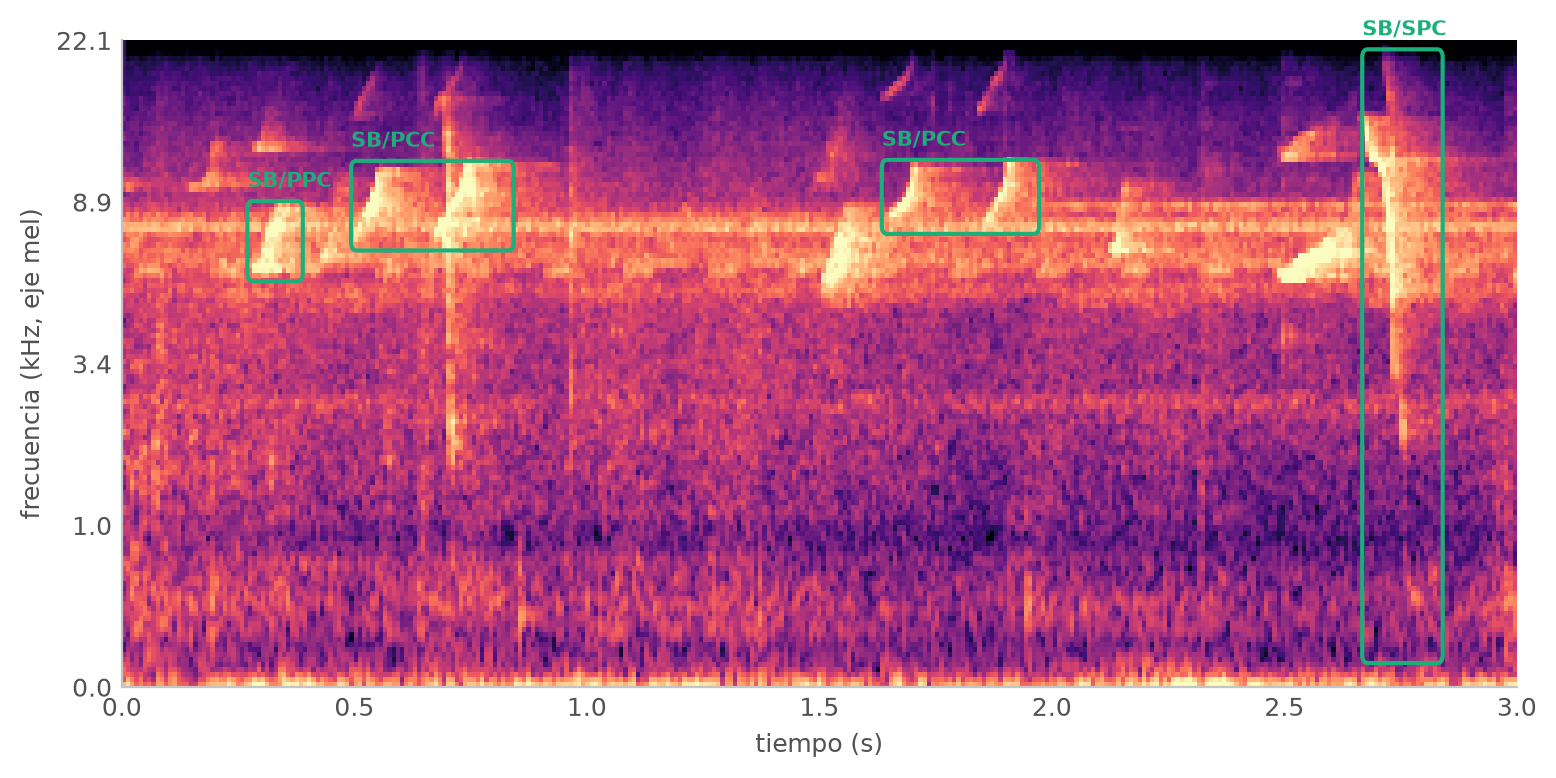
\includegraphics[width=0.98\textwidth]{window_example.png}
      \par\medskip
      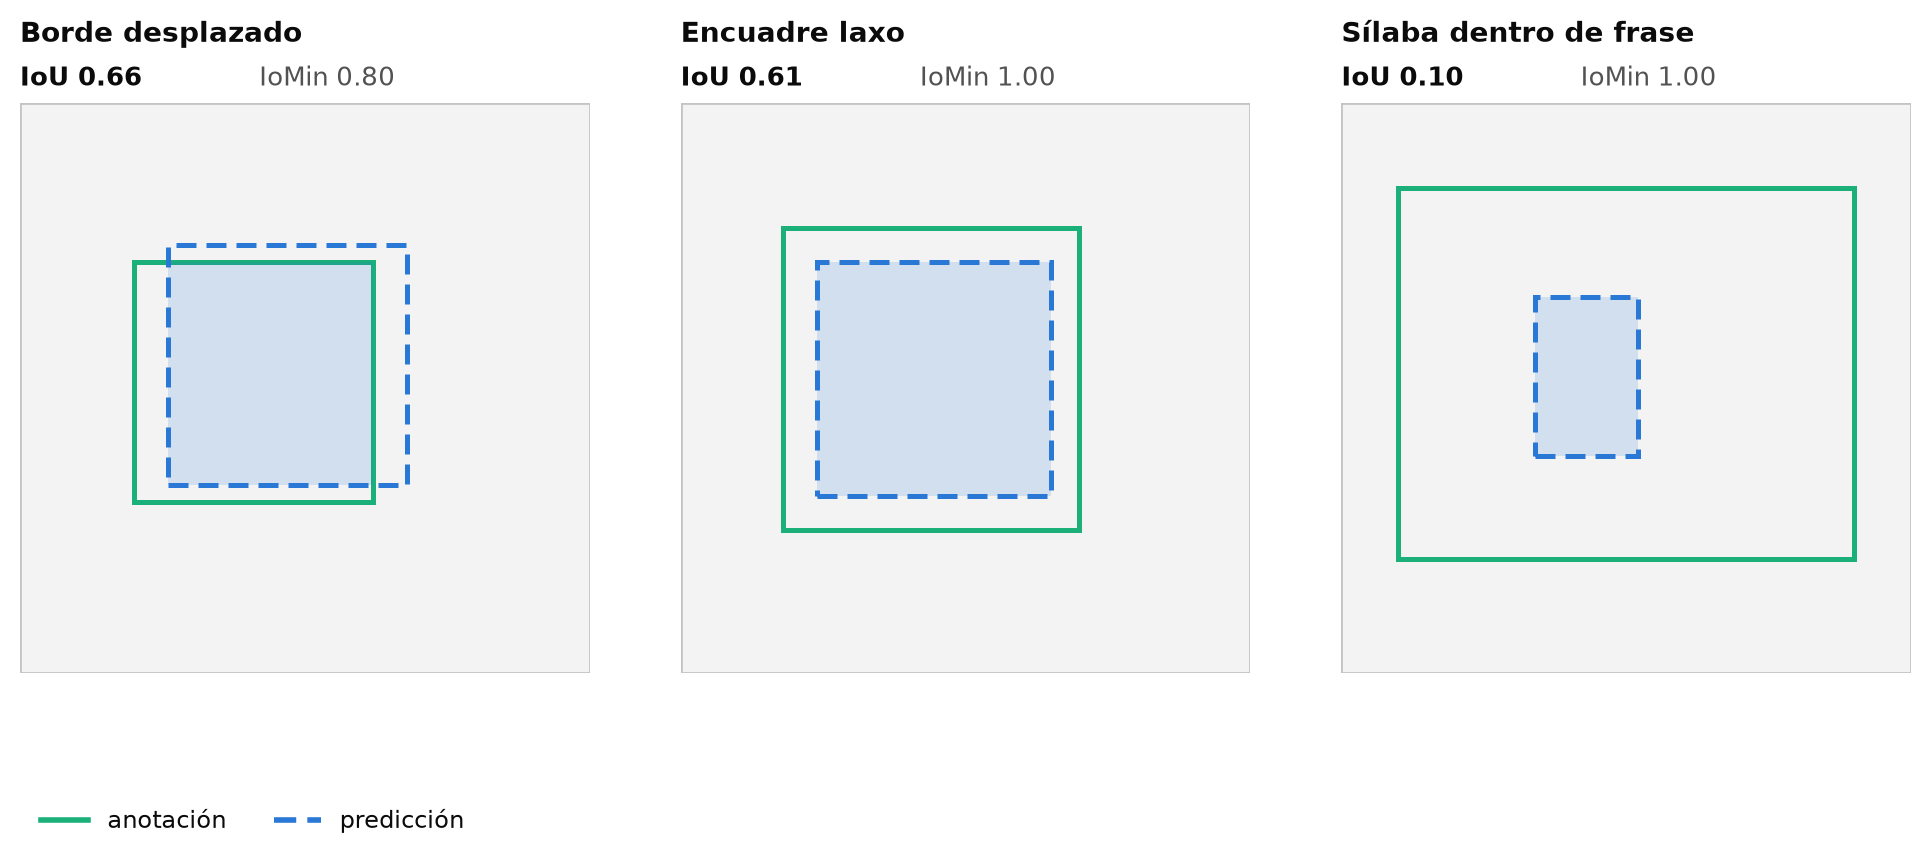
\includegraphics[width=0.98\textwidth]{iou_criterion.png}
    \end{column}
  \end{columns}
\end{frame}

% ===================================================================
\begin{frame}{El Desbalance de clases}
  \begin{columns}[T]
    \begin{column}{0.62\textwidth}
      \centering
      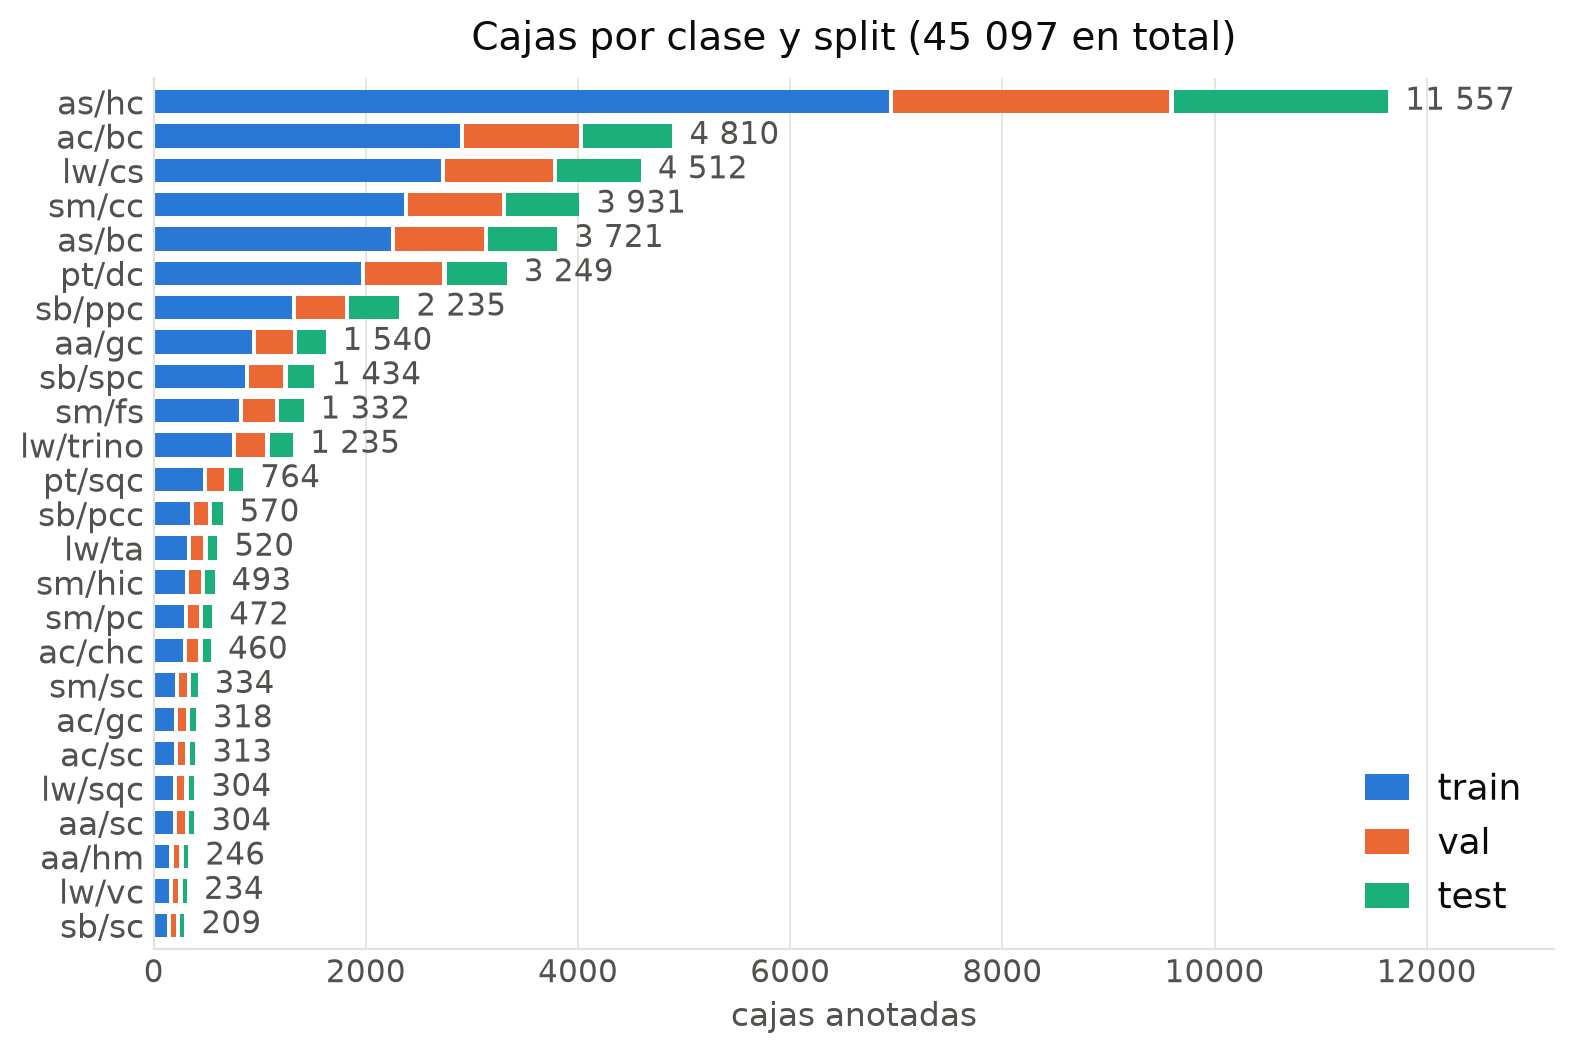
\includegraphics[width=\textwidth]{dataset_support.png}
    \end{column}
    \begin{column}{0.36\textwidth}
      \footnotesize
      \begin{itemize}
        \item \texttt{as/hc} (aullido de \textit{Alouatta}) aporta \textbf{2\,023}
              cajas de test; \texttt{sb/sc} sólo \textbf{37}. Un factor de 55.
        \item Ocho clases tienen menos de 100 cajas de test.
        \item Las llamadas \textbf{largas y tonales} abundan; los \textit{squeaks} y
              \textit{chirps} de decenas de milisegundos son minoría y son,
              además, los más difíciles de encuadrar.
      \end{itemize}
      \medskip
      \gris{Este reparto es el que explica el piso por clase que aparece en los
      resultados: no es sólo un problema de modelo.}
    \end{column}
  \end{columns}
\end{frame}

% ===================================================================
\begin{frame}{Arquitecturas comparadas}
  \centering
  \small
  \begin{tabular}{@{}lcccc@{}}
    \toprule
     & \textbf{\color{cFRCNN}Faster R-CNN} & \textbf{\color{cDETR}DETR ts5}
     & \textbf{\color{cDETRb}DETR ts10} & \textbf{\color{cYOLO}YOLO26} \\
    \midrule
    Backbone             & ResNet-50      & AST            & AST            & CSP propio \\
    Preentrenamiento     & COCO           & AudioSet        & AudioSet        & COCO \\
    Parámetros           & 43,4 M         & 89,6 M          & 89,6 M          & 10,0 M \\
    \gris{entrenables}   & \gris{43,4 M}  & \gris{3,1 M}    & \gris{3,1 M}    & \gris{10,0 M} \\
    Cajas candidatas     & RPN + 100      & 64 queries      & 64 queries      & 300 (end-to-end) \\
    Entrada              & $3\times416\times1024$ & $1\times128\times331$
                         & $1\times128\times331$ & $3\times512\times512$ \\
    Tokens / resolución  & ---            & $12\times64$ · 47 ms
                         & $12\times32$ · 94 ms & --- \\
    Elección del \textit{best} & F3 (val) & F3 (val)        & F3 (val)
                         & \textbf{mAP@0,5:0,95} \\
    \bottomrule
  \end{tabular}

  \medskip
  \begin{block}{Lo que está igualado para los cuatro}
    \small Mismas ventanas y mismo split · score $\geq$ 0,5 · IoU $\geq$ 0,5 ·
    supresión de anidadas a 0,3 · tope de 64 detecciones por ventana ·
    \texttt{box\_score\_thresh} 0,001 · una sola implementación de las métricas.
    \textbf{No} está igualada la receta de entrenamiento: cada framework corre con la
    suya, y YOLO26 elige su \textit{checkpoint} con otro criterio.
  \end{block}
\end{frame}

% ===================================================================
\begin{frame}{Resultados}
  \centering
  \small
  \begin{tabular}{@{}llccccc@{}}
    \toprule
    & & \textbf{Recall} & \textbf{Precisión} & \textbf{F3}
    & \textbf{mAP@0,5} & \textbf{mAP@0,5:0,95} \\
    \midrule
    \frcnn & val  & 0,770 & 0,500 & 0,731 & 0,474 & 0,205 \\
                            & test & \textbf{0,777} & 0,499 & \textbf{0,736} & 0,487 & 0,211 \\
    \addlinespace
    \detrA                  & val  & 0,694 & 0,532 & 0,674 & 0,362 & 0,136 \\
                            & test & 0,694 & 0,517 & 0,671 & 0,373 & 0,143 \\
    \addlinespace
    \detrB                  & val  & 0,677 & 0,521 & 0,657 & 0,357 & 0,138 \\
                            & test & 0,682 & 0,499 & 0,658 & 0,347 & 0,138 \\
    \addlinespace
    \yolo                   & val  & 0,533 & 0,819 & 0,552 & 0,531 & 0,263 \\
                            & test & 0,532 & \textbf{0,805} & 0,550 & \textbf{0,520} & \textbf{0,264} \\
    \bottomrule
  \end{tabular}

  \medskip
  \footnotesize
  \begin{columns}[T]
    \begin{column}{0.33\textwidth}
      \textbf{Punto de operación} \gris{(F3)}\\
      Faster R-CNN $>$ DETR $\gg$ YOLO26
    \end{column}
    \begin{column}{0.33\textwidth}
      \textbf{Curva completa} \gris{(mAP)}\\
      YOLO26 $>$ Faster R-CNN $\gg$ DETR
    \end{column}
    \begin{column}{0.33\textwidth}
      \textbf{val $\rightarrow$ test}\\
      sin caída: máx.\ 0,007 de recall
    \end{column}
  \end{columns}
  \medskip
  \gris{Faster R-CNN gana el recall en 24 de 25 clases; la mAP baja de los DETR
  (0,14) delata un encuadre flojo.}
\end{frame}

% ===================================================================
\begin{frame}{Recall-precisión}
  \begin{columns}[T]
    \begin{column}{0.56\textwidth}
      \centering
      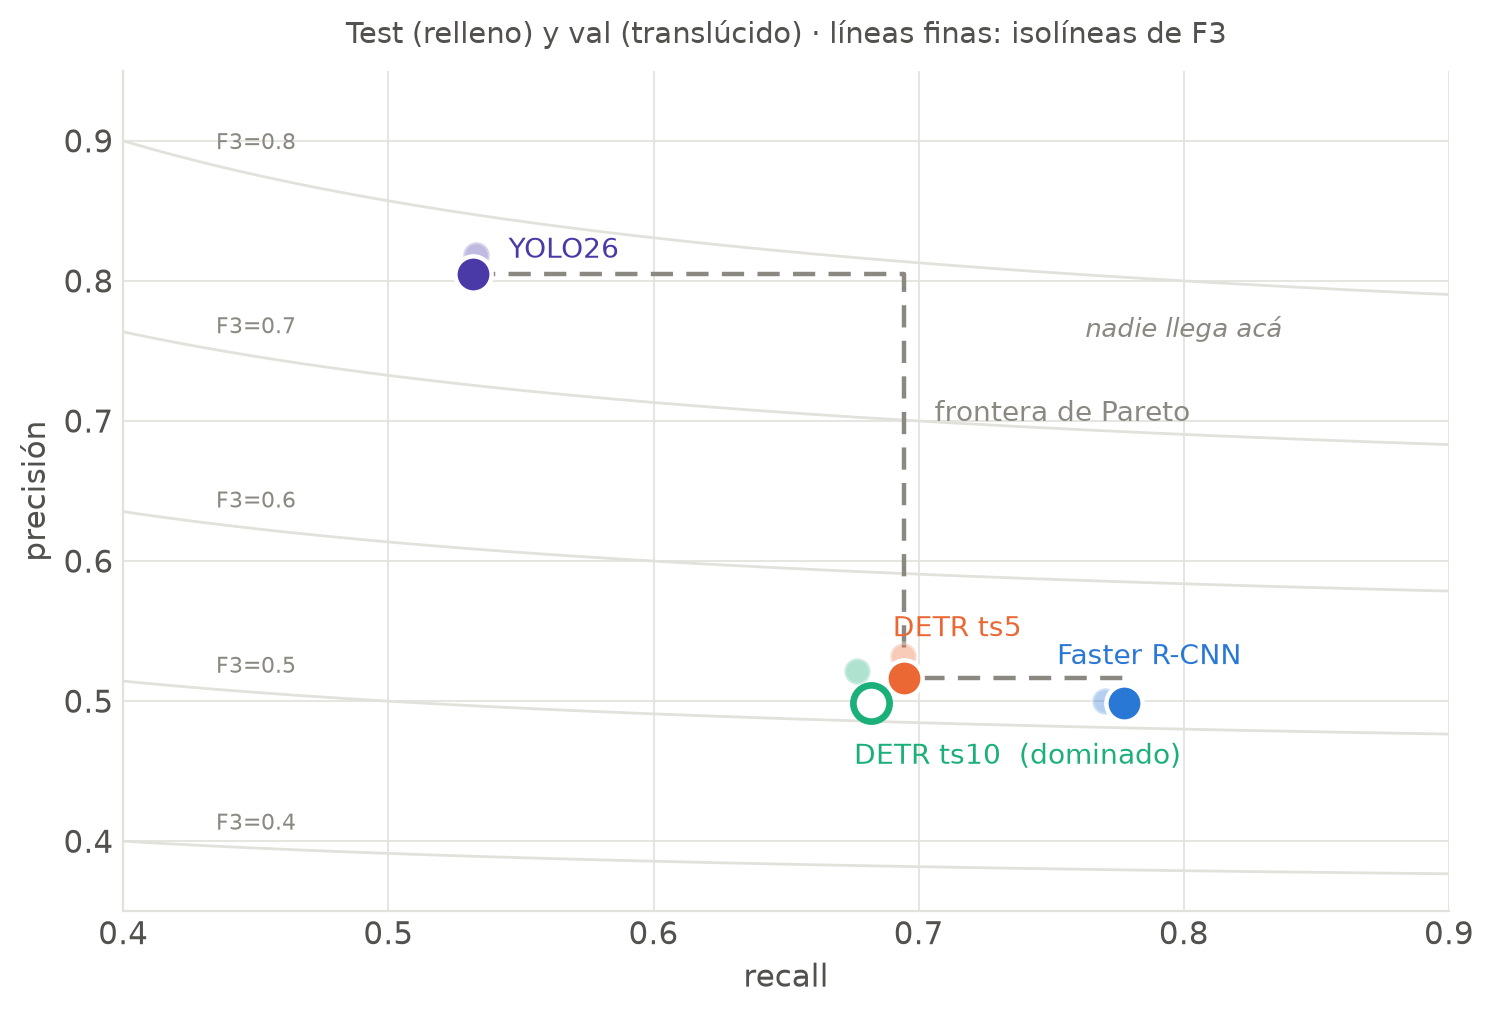
\includegraphics[width=\textwidth]{pr_plane.png}
    \end{column}
    \begin{column}{0.42\textwidth}
      \footnotesize
      \textbf{Tres modelos no dominados}; elegir entre ellos es una decisión de uso,
      no de calidad:
      \begin{itemize}
        \item \frcnn{} --- máximo recall (0,777): 2 cajas revisadas por llamada
              recuperada, y casi nada se pierde.
        \item \detrA{} --- intermedio, con sólo \textbf{3,1 M} de parámetros
              entrenables.
        \item \yolo{} --- máxima precisión (0,805) con 10 M de parámetros; deja
              fuera casi la mitad de las llamadas.
      \end{itemize}
      \smallskip
      \textbf{\detrB{} está dominado} por ts5: menos recall \textit{y} menos
      precisión. Es lo único que la ablación descarta sin ambigüedad.
      \smallskip
      \gris{Con F3 --- el criterio de la tesis, recall $\times 9$ --- el orden es
      Faster R-CNN, DETR, YOLO26.}
    \end{column}
  \end{columns}
\end{frame}

% ===================================================================
\begin{frame}{Limitaciones de cada enfoque}
  \scriptsize
  \begin{columns}[T]
    \begin{column}{0.49\textwidth}
      \textbf{\color{cFRCNN}Faster R-CNN --- el mejor hoy}
      \begin{itemize}
        \item Precisión 0,499: la mitad de lo que propone se descarta a mano.
        \item Entrena sus 43,4 M de parámetros desde COCO: no aprovecha ningún
              preentrenamiento de audio.
        \item mAP@0,5:0,95 de 0,211: el encuadre sigue flojo.
      \end{itemize}
      \medskip
      \textbf{\color{cDETR}DETR (AST congelado) --- la arquitectura propia}
      \begin{itemize}
        \item 3,1 M entrenables: recall competitivo, pero mAP la mitad que la de
              Faster R-CNN.
        \item Su recall por clase sigue al soporte ($\rho = 0{,}56$): las clases
              raras no llegan a aprenderse.
        \item Bajar el paso de 10 a 5 cuesta $4\times$ y devuelve $+0{,}012$ de recall.
      \end{itemize}
    \end{column}
    \begin{column}{0.49\textwidth}
      \textbf{\color{cYOLO}YOLO26 --- el más barato}
      \begin{itemize}
        \item Recall 0,532: 13 de 25 clases por debajo de 0,35.
        \item Su \textit{checkpoint} se eligió por mAP@0,5:0,95, no por F3: el punto
              de operación está sin calibrar, es un piso.
        \item Sin preentrenamiento de audio.
      \end{itemize}
      \medskip
      \textbf{\color{cMuted}Transversal --- lo que no sostiene ningún número}
      \begin{itemize}
        \item \textbf{Una sola semilla} por corrida: diferencias menores a
              $\sim0{,}01$ de mAP no se separan del ruido.
        \item Ablación incompleta: falta el paso 2, la rama \texttt{logmel} y el
              \textit{fine-tune} del AST. El PCEN aún no es un número.
        \item \textbf{EAT + DINO} implementado y verificado, pero sin entrenar.
      \end{itemize}
    \end{column}
  \end{columns}
\end{frame}

\begin{frame}[standout]
  Gracias
\end{frame}

\end{document}
